\subsection{Wägezelle}

Wägezellen messen mechanische Verformungen.
Wird auf eine Wägezelle eine Gewichtskraft \mbox{$F = m \cdot g \: [\frac{kg \cdot m}{s^2}]$} (m = aufgebrachte Masse und $g = 9.81 \: \frac{m}{s^2}$)  aufgebracht, verformt sich diese unter der Krafteinwirkung.
Auf der Wägezelle sind Dehnungsmessstreifen aufgebracht, deren Widerstand sich bei Verformung ändert.
Die Dehnungsmessstreifen sind in einer Wheatstone-Brücke verschaltet, die die Widerstandsänderung in eine Spannungsänderung umwandelt, die meist nur im Bereich weniger Millivolt liegt.
Diese Spannungsänderung ist proportional zur aufgebrachten Gewichtskraft.
Unten dargestellt in \autoref{CAD-Darstellung-Waegezelle} ist der Aufbau einer Wägezelle als CAD-Modell. \\
\begin{figure}[h!]
    \centering
    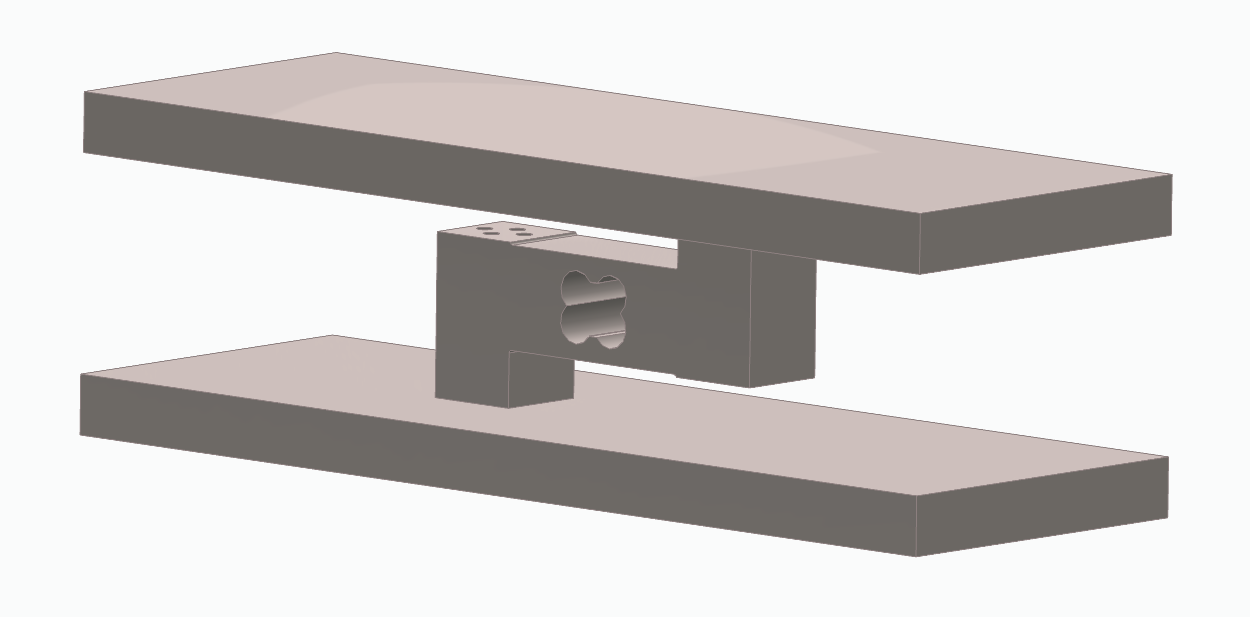
\includegraphics[width=0.9\textwidth]{img/CAD_Waegezelle.png}
    \caption{CAD Darstellung Wägezelle}
    \label{fig:CAD-Darstellung-Waegezelle}
\end{figure}

\begin{figure}[h!]
    \centering
    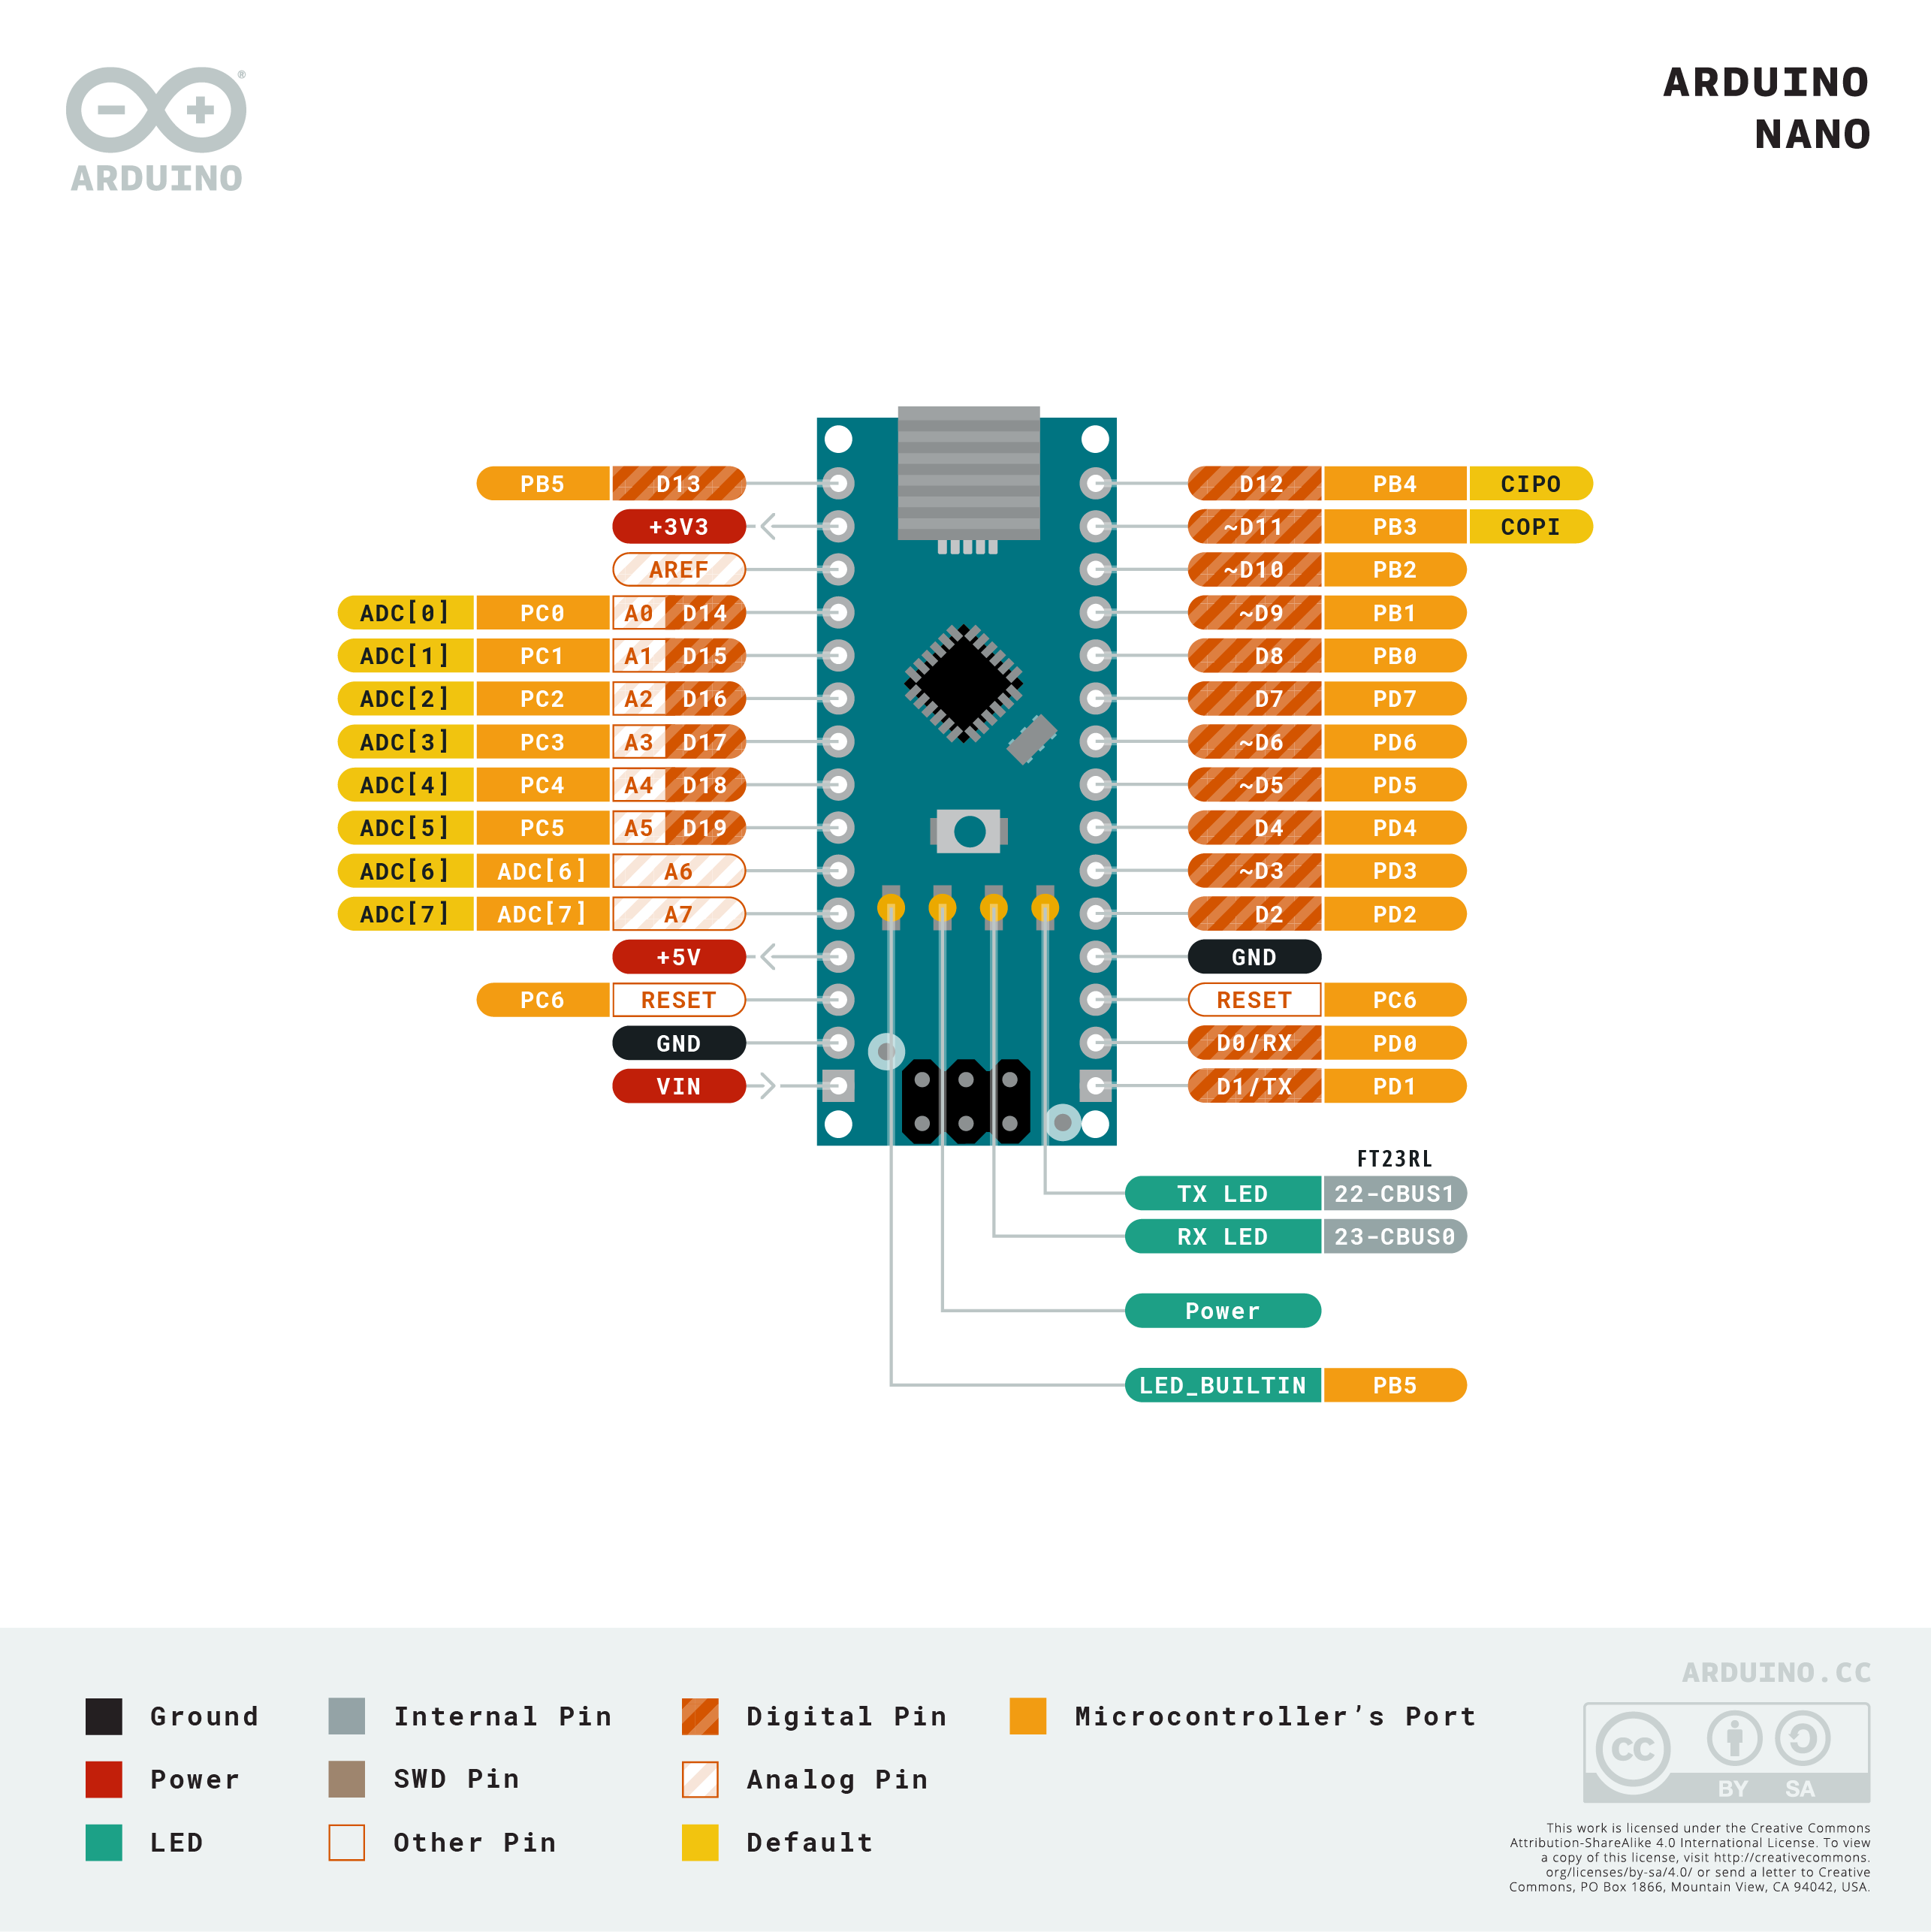
\includegraphics[width=0.9\textwidth]{img/Nano-Pinlayout.png}
    \caption{Nano-Pinlayout \cite{Arduino}}
    \label{fig:Nano-Pinlayout}
\end{figure}

\begin{figure}[h!]
    \centering
    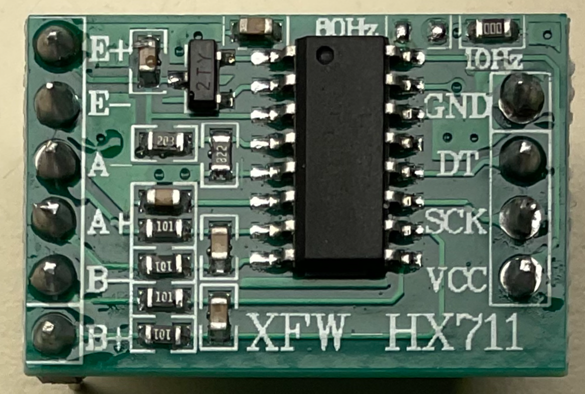
\includegraphics[width=0.6\textwidth]{img/HX711.png}
    \caption{HX711 \cite{prilchen}}
    \label{fig:HX711}
\end{figure}

\begin{figure}[h!]
   \centering
   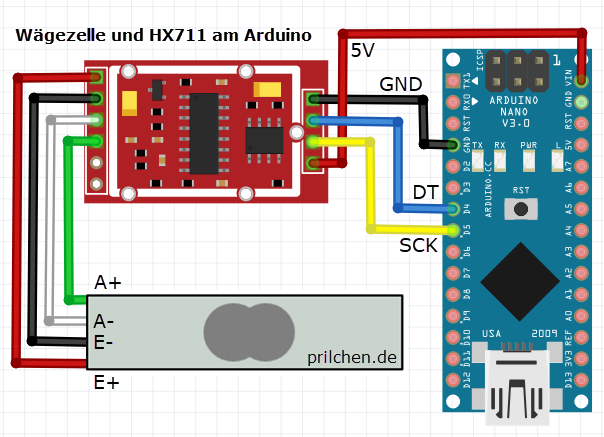
\includegraphics[width=0.6\textwidth]{img/waegezelle_verschaltung.png}
   \caption{HX711 Schaltung mit Arduino Nano \cite{prilchen}}
   \label{fig:HX711-Nano-Schaltung}
\end{figure}


Um die Signale der Wägezelle an den HX711 weiterzugeben und die Signale des HX711 mit dem Arduino Nano verarbeiten und die Daten lesbar darzustellen, müssen die drei Komponenten miteinander verschaltet werden und korrekt kommunizieren. \\
Zuerst wird die Wägezelle an eine 5 V Gleichstromquelle angeschlossen und dann mit dem HX711 verbunden. Wodurch die Wägezelle die analogen Signale an den HX711 weitergeben kann. Der HX711 wandelt sie dann in ein digitales Signal und gibt dieses an den Arduino Nano weiter.
Der VCC-Pin HX711 wird mit dem 5V-Pin des Arduino Nano verbunden. Der GND-Pin mit dem GND-Pin des Ardiunos. Der DT-Pin ist der Datenausgang des HX711 und wird mit irgendeinem der Digital-Pins des Nanos verbunden, genauso wie der SCK-Pin, z.B. $DT-Pin -> D3-Pin$ und $SCK-Pin -> D2-Pin$. Der SCK-Pin oder serial-clock-Pin steuert die Übertragung des Signals des DT-Pins.
Der Arduino gibt auf dem SCK-Pin den Takt vor, mit dem der HX711 die Daten an den Mikrocontroller sendet.
Der Ardiuno setzt den SCK-Pin auf high und dann wieder auf low. Dieser Wechsel, vom Ende eines low-Signals zu einem high- und wieder einem low-Signal ist ein Takt.
Der HX711 sendet dann pro Takt ein Bit, also einen low-Puls für 0 und einen high-Puls für 1. \\
\\
Der Arduino-Nano wird dann an einen Computer angeschlossen.
In der Arduino IDE können mithilfe der passenden Library und einem Code die Daten ausgelesen und gespeichert werden.
\\
\\
Der auf dem Arduino ausgeführte C-Code liest periodisch den analogen Wert des HX711 aus. Zunächst muss der Sensor initialisiert werden. Dies geschieht durch:
\begin{enumerate}
    \item \textbf{Angabe eines Kalibrationswertes}: Dieser Wert dient der genauen Gewichtsmessung.
    \item \textbf{Tara-Einstellung}: Die Waage wird auf 0 kg gesetzt, um sicherzustellen, dass nachfolgende Messungen korrekt sind.
\end{enumerate}
Nach der Initialisierung ist die Waage bereit, Messdaten auszugeben.
\\
Für die Ausgabe eines Messwerts werden die gemessenen Daten über den Serial-Port übertragen.
Dabei wird angegeben, ob die Messung von der linken oder rechten Waage stammt.
Die Ausgabe erfolgt beispielsweise wie folgt:
\begin{center}
    \texttt{Gewicht rechts [kg]: -0.00118}  \\
    \texttt{Gewicht links [kg]: -0.00321} \\
    \texttt{Gewicht rechts [kg]: -0.00118} \\
    \texttt{Gewicht links [kg]: -0.00223} \\
\end{center}
Der serielle Monitor verarbeitet die Ausgabe des Arduinos und ergänzt jeden Messwert mit einem Zeitstempel, der den Zeitpunkt angibt, zu dem der Messwert den Computer erreicht. Dadurch wird es möglich, die seriellen Daten in Echtzeit als Graph über die Zeit darzustellen, wie in Abbildung \ref{fig:serial_output} veranschaulicht.
%todo:
\begin{figure}[h!]
    \centering
    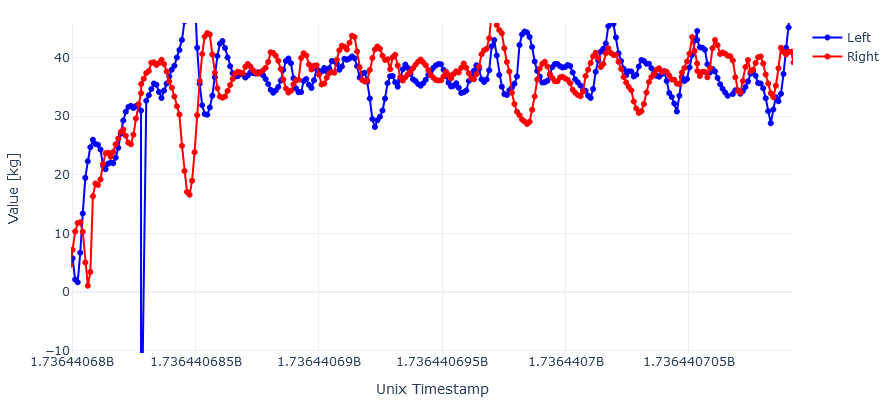
\includegraphics[width=0.7\textwidth]{img/serial_output_example.png} % Screenshot oder Beispiel
    \caption{Ausgabe der Messdaten mit Python}
    \label{fig:serial_output}
\end{figure}
\\
Allen Daten werden in einem CSV-Format gespeichert.
Sie können nun beliebig aufbereitet und analysiert werden.
% Der C Code auf dem Arduino liest periodisch den analogen Wert des HX711 aus, muss dafür aber zuerst initialisiert werden.
% Dazu wird ein Kalibrationswert angegeben und anschließend die Waage auf 0 kg getared.
% Nun ist die Waage initialisiert und bereit, Messdaten auszugeben.
% Soll ein Messwert ausgegeben werden, so werden die Daten an den Serial-Port ausgegeben, mit dem Hinweis, ob der Messwert von links oder rechts stammt.
% \begin{center}
%     Gewicht links: ...  \\
%     Gewicht rechts: ...
% \end{center}
% An dem Serial-Port angekommen werden die Daten von einem zweiten parallel laufenden Python Skript ausgewertet.
% Dabei können die Daten in Echtzeit in einer web App dargestellt werden und werden gleichzeitig aufgezeichnet im CSV-Format.
% \\
% Diese Daten können nun auf verschiedene Art und Weisen mithilfe von Python dargestellt werden.






\subsection{Elektromyographie}

Mit einem EMG kann die elektrische Muskel-Aktivität gemessen werden.

Dazu wird die elektrische Aktivität in einem ruhenden und einem kontrahierten Muskel gemessen. Das Signal entsteht aus dem Aktionspotential der Muskelfasermembran und dem Depolarisations- und Repolarisationsverlauf, der in \autoref{fig:Depolarisations-und-Repolarisationsverlauf} als Funktion der Zeit dargestellt ist. Im Ruhetonus liegt das Potential zwischen $-80$ und  $-90$ mV.

\begin{figure}[h!]
    \centering
    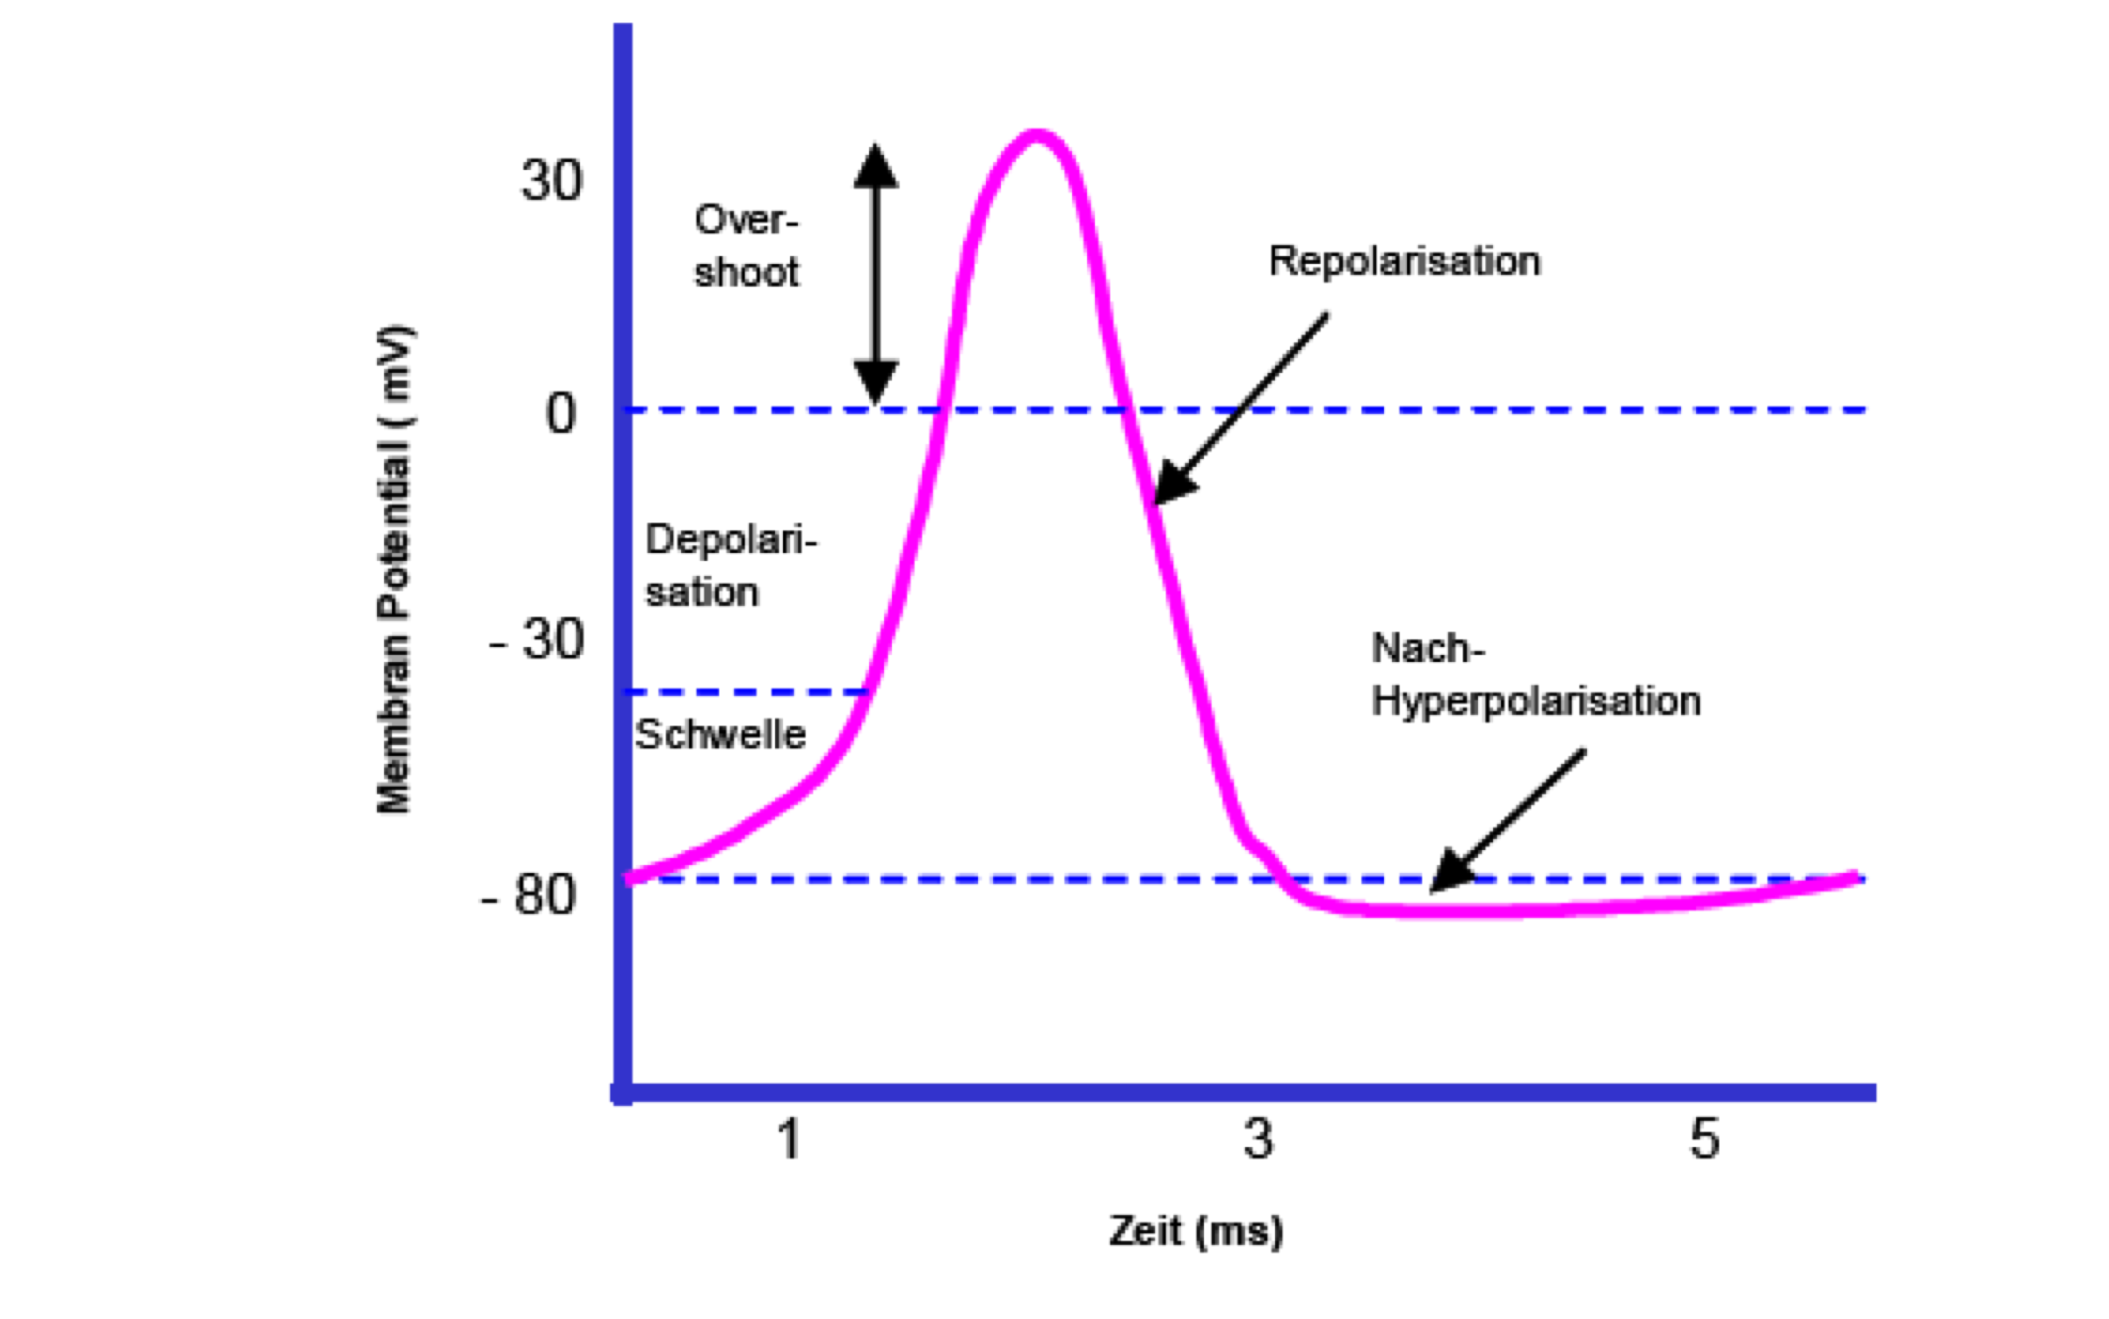
\includegraphics[width=0.8\textwidth]{img/De-Repolarisation.PNG}
    \caption{De- und Repolarisation und Aktionspotential Muskelfasermembran \cite{Vorlesung-Muskulatur-EMG}}
    \label{fig:depolarisations-und-repolarisationsverlauf}
\end{figure}

Eine Muskelkontraktion startet auf Sarkomerebene.
Durch das Zusammenwirken aller Sarkomere wird die Umwandlung von chemischer Energie in mechanische Energie als Kontraktion des Muskels sichtbar.
\\
\\
Ein  Nervenimpuls gelangt als Aktionspotential über das Axon eines Motoneurons zum Axonende. \\
Durch Neurotransmitter die in den postsynaptischen Spalt ausgeschüttet und dann an den Rezeptor der postsynaptischen Membran binden, wird der Prozess der Depolarisation in der Muskelfaser ausgelöst, der auf der linken Seite von  \autoref{fig:depolarisations-und-repolarisationsverlauf} dargestellt ist:\\
\\
Der Rezeptor ist ein Kanal für Kationen, also positiv geladene Ionen wie Natrium-, Calcium- oder Kaliumionen. Wird der Ionenkanal geöffnet, kommt es zum Einfluss von Kationen und zu einer  Depolarisation der Muskelfaser. Wird ein gewisses Schwellenpotential überschritten, öffnen sich spannungsabhängige Natrium-Kanäle, wodurch ein Aktionspotential ausgelöst wird, das als EMG-Signal gemessen werden kann.
In \autoref{fig:depolarisations-und-repolarisationsverlauf} als Schwelle gekennzeichet, ab der die Steigung der Potential-Funktion zunimmt, bis die Funktion bis $+20$ bis $+30$ mV steigt.
Das Aktionenpotential löst nun wiederum die Öffnung von spannungsgesteuerten Calcium-Kanälen aus, wodurch Calcium-Ionen in der Muskelfaser freigesetzt werden. Es kommt zu einer Anhäufung von Calcium-Ionen in der Muskelfaser. Dadurch steigt Calciumkonzentration, was die Kontraktion der Muskelfaser auslöst. \\
Noch bevor der Höhepunkt des Aktionspotentials erreicht ist, werden die Natriumkanäle inaktiv und positiv geladene Kalium strömen aus der Zelle. Das Potential nähert sich nach einer Hyperpolarisationsphase, während der das Pontential unter das Ruhepotential von $-80$ mV fällt, wieder dem Ruhepotential an.

Die EMG-Messung findet in der Hochschule im Labor für Ergonomie statt.
Die Daten werden mithilfe eines Programms von NORAXON ausgelesen und analysiert.


